\chapter{Сеанс работы в Linux}

\section{Задание}
	Определение понятий и анализ работы ниже названных объектов и процессов, которые происходят при сеансе работы в Linux:
\begin{itemize}
	\item Загрузка системы, ядро ​​системы, регистрация в системе, имя входящего пользователя.
	\item Персональный компьютер, многопользовательская операционная система, 					пользователи, администраторы, домашний каталог.
	\item Учетная запись UID, GID, полное имя, командная оболочка, интерпретатор командной 	строки, задачи администратора и его UID и GID.
	\item Хост, пароль, приглашение командной строки, идентификация.
	\item Виртуальные консоли их интерфейс, вызов виртуальных консолей и работа в них.
	\item Графические консоли.
	\item Имя пользователя, сеанс работы в системе, выходной поток данных, выход из 			системы.
\end{itemize}

\section{Основная часть}
	Обработка работы команд:
\begin{enumerate}
	\item Регистрация в системе.
	\begin{figure}[h]
		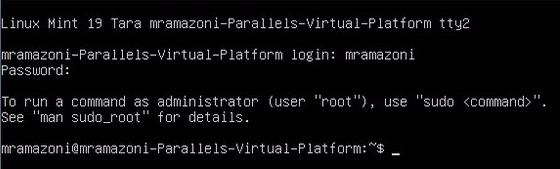
\includegraphics{lab1_2.png}
		\centering
	\end{figure}
	\newpage
	\item Изменение пароля.
	\begin{figure}[h]
		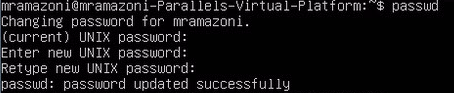
\includegraphics{lab1_3.png}
		\centering
	\end{figure}
	\item Определение учетной записи пользователя от имени которого выполняется работа.
	\begin{figure}[h]
		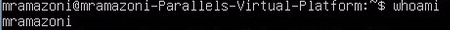
\includegraphics{lab1_4.png}
		\centering
	\end{figure}
	\item Вывод списка пользователей, которые в данный момент зарегистрированых в системе.
	\begin{figure}[h]
		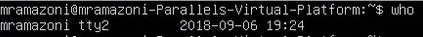
\includegraphics{lab1_5.png}
		\centering
	\end{figure}
	\item Вывод информации о пользователях, работавших в системе.
	\begin{figure}[h]
		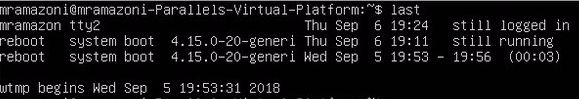
\includegraphics{lab1_6.png}
		\centering
	\end{figure}
	\item Выход из системы.
	\begin{figure}[h]
		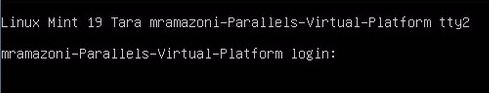
\includegraphics{lab1_1.png}
		\centering
	\end{figure}
\end{enumerate}

\section{Выводы}
	Ядро Linux (/ˈlɪnʊks/) — ядро операционной системы, соответствующее стандартам POSIX, составляющее основу операционных систем семейства Linux.
	
	
	Виртуальная консоль — это системная консоль компьютера, где пользователь может переключаться из одной виртуальной консоли в другую для произведения множества независимых действий.
	
	
	Интерфейс командной строки (англ. Command Line Interface, CLI). - управление программами с помощью команд. Команды состоят из букв, цифр, символов, набираются построчно, выполняются после нажатия клавиши Enter.
	
	
	Во время загрузки Ubuntu запускаются семь полноэкранных консолей, у каждой свой независимый сеанс, с первой по шестую с интерфейсом командной строки, в седьмой запускается графический режим.


	Переключиться на одну из виртуальных консолей можно нажав сочетание клавиш:
\begin{itemize}
 
	\item Ctrl+Alt+F1 - первая виртуальная консоль; 
	\item Ctrl+Alt+F2 - вторая виртуальная консоль; 
	\item Ctrl+Alt+F3 - третья виртуальная консоль; 
	\item Ctrl+Alt+F4 - четвертая виртуальная консоль; 
	\item Ctrl+Alt+F5 - пятая виртуальная консоль; 
	\item Ctrl+Alt+F6 - шестая виртуальная консоль; 
	\item Ctrl+Alt+F7 - седьмая виртуальная консоль, возврат в графический режим. 

\end{itemize} 


	После запуска терминала мы видим строку с приглашением к вводу команд, например: 
mramazoni@mramazoni-Parallels-Virtual-Platform:~\$ 
\begin{itemize}

	\item mramazoni - имя учетной записи пользователя
	\item @ - разделитель между учетной записью и именем компьютера 
	\item mramazoni-Parallels-Virtual-Platform - имя компьютера 
	\item : - разделитель 
	\item ~ - в какой папке выполняется команда, ~ это домашняя папка пользователя
	\item \$ - приглашение к выполнению команды с правами простого пользователя (# будет 		означать приглашение на выполнение команд с правами администратора)

\end{itemize}
